\documentclass[11pt]{article}
\usepackage[margin=1in]{geometry}
\usepackage{amsmath,amssymb,amsthm}
\usepackage{hyperref}
\usepackage{graphicx}
\usepackage{mathtools}
\usepackage{physics}
\usepackage{bm}
\usepackage{microtype}
\usepackage{enumitem}

\title{Dynamic Index Budget and Cosmological Phase Transitions}
\author{Matthew Sandoz}
\date{\today}

\theoremstyle{plain}
\newtheorem{theorem}{Theorem}[section]
\newtheorem{lemma}[theorem]{Lemma}
\newtheorem{proposition}[theorem]{Proposition}
\newtheorem{corollary}[theorem]{Corollary}
\theoremstyle{definition}
\newtheorem{definition}[theorem]{Definition}
\newtheorem{remark}[theorem]{Remark}
\newtheorem{postulate}[theorem]{Postulate}
\newcommand{\Inv}{^{-1}} % Alternatively, defines \Inv as a shorthand for ^{-1}

\graphicspath{{./}{/mnt/data/}}

\begin{document}
\maketitle
\begin{abstract}
  We formalize the ``Dynamic Index Budget'' hypothesis: the idea that cosmological evolution is constrained by a time-dependent bound on the local Jones index density of the spin network. We derive an instability theorem for over-budget states, show how matter condensation emerges as an optimal index-allocation problem, and outline falsifiable predictions for particle spectra and cosmological observables.
\end{abstract}

\section{Introduction}
In the operator-algebraic formulation of spin networks, the local Jones index $[N':N]$ measures the capacity of a boundary to support bridge processes. We propose that this capacity is subject to a cosmological budget $I_B(t)$ which decreases monotonically with cosmic expansion.

\paragraph{From static area caps to a dynamic budget.}
Locally, bridge insertions increase boundary entropy by $\Delta S=\ln(2j+1)$ per conduit and are limited by the minimal cut area (in the same units), cf.\ the Index Budget Bound $\prod_a(2j_a+1)\le e^{\mathrm{Area}_{\mathrm{cut}}}$.
In the present work we promote this static cap to a time-dependent budget $I_B(t)$ that reflects cosmological conditions (dilution, modular temperature, matter density). Thus, the \emph{Dynamic Index Budget} hypothesis is the spacetime evolution of those local caps, constraining when and where stable condensates (particles) can form.

\section{Evolution Equation for the Dynamic Index Budget}\label{sec:budget-evolution}

We promote $I_B(t)$ to a dynamical field with a coarse-grained evolution law that couples to expansion and matter content:
\begin{equation}
  \boxed{\quad
    \frac{d I_B}{dt}
    =
    -\,\alpha_H\,H(t)\,I_B(t)\;
    -\;\alpha_s\,s(t)\;
    -\;\alpha_\chi\,\Theta(t)\;
    +\;\mathcal{S}_{\rm micro}(t)
  \quad}
  \label{eq:IB-evolution}
\end{equation}
where:
\begin{itemize}[leftmargin=*]
  \item $H(t)$ is the Hubble rate; the term $-\alpha_H H I_B$ captures dilution of local index capacity by cosmic expansion.
  \item $s(t)$ is the entropy density of matter/radiation; $-\alpha_s s(t)$ accounts for \emph{screening} of bridge capacity by thermal disorder.
  \item $\Theta(t)=\sum_i \nu_i\,\rho_i(t)$ is a weighted matter functional (e.g.\ over energy densities $\rho_i$ with weights $\nu_i$ set by coupling strengths); $-\alpha_\chi \Theta$ models index \emph{drag} from ambient couplings.
  \item $\mathcal{S}_{\rm micro}(t)$ is a source term from microrearrangements that \emph{return} budget (e.g.\ topology–simplifying rewrites or decays).
\end{itemize}

The coefficients $(\alpha_H, \alpha_s, \alpha_\chi)$ are determined from the
singular spectrum of the one–cell transfer map: the leading singular modes
set the baseline dilution rate $\alpha_H$, entropy screening $\alpha_s$,
and matter–coupling drag $\alpha_\chi$ through their respective projection
weights on expansion, disorder, and coupling channels.

All coefficients $(\alpha_H,\alpha_s,\alpha_\chi)$ are positive and, in our operator setting,
are determined by the one–cell transfer map and local rewrite statistics;
see Appendix~\ref{app:transfer-numerics} for how $\kappa$ and singular spectra fix these scales.
In eras with negligible source, \eqref{eq:IB-evolution} reduces to
\(
  \dot I_B \approx -(\alpha_H H + \alpha_s s/I_B + \alpha_\chi \Theta/I_B)\, I_B,
\)
so $I_B$ decays multiplicatively with expansion and additively with matter/entropy loading.

\paragraph{Connection to Standard Cosmology.}
For standard $\Lambda$CDM cosmology, the Dynamic Index Budget predicts distinct
thresholds aligning with known thermal epochs:
\begin{itemize}[leftmargin=*]
  \item \textbf{Electroweak epoch:} $I_B \approx 1.10$ at $T \approx 100~\mathrm{GeV}$,
    corresponding to the index cost of a single spin-1 bridge.
  \item \textbf{QCD confinement epoch:} $I_B \approx 2.08$ at $T \approx 200~\mathrm{MeV}$,
    corresponding to the combined cost of three spin-$\tfrac12$ bridges.
\end{itemize}
These thresholds mark the onset of stable condensation for the associated
particle families and are consistent with observed relic abundances.

\section{Collective States and Index Budgets}
\subsection{Index Budget from Fusion Rules}
The maximum local index density is bounded by the quantum group level:
\begin{equation}
  \rho_I \leq \ln(k+2)
\end{equation}
per unit area, where $k$ is the $\mathrm{SU}(2)_k$ level parameter.
\begin{definition}[Pre-Geometric State $G_0$]
  A maximally connected spin network with:
  \begin{itemize}
    \item No stable particles ($\tau \ll \Gamma_{\mathrm{env}}^{-1}$ for all structures)
    \item Maximal relational entropy dominated by virtual bridges.
  \end{itemize}
\end{definition}

\subsection{Local Index Density (Unified Definition)}\label{subsec:rhoI-unified}
Let $G$ be a spin network and $R\subset G$ a region with boundary $\partial R$. The \emph{local index density} is
\begin{equation}
  \rho_I(R)
  \;:=\;
  \frac{1}{\mathrm{Area}(\partial R)}\,
  \sum_{P\subset R} \Delta S_P
  \;=\;
  \frac{1}{\mathrm{Area}(\partial R)}\,
  \sum_{P\subset R} \ln [N':N]_P,
  \label{eq:rhoI-unified}
\end{equation}
where the sum runs over bridge processes $P$ whose inclusions cross $\partial R$ and $\Delta S_P=\ln [N':N]_P$ is the Jones–index entropy jump for $P$. The dynamic budget imposes $\rho_I(R)\le I_B(t)$ for all $R$.
\begin{remark}[Local Index Density]
  For a region $R$,
  \begin{equation}
    \rho_I(R) = \frac{1}{\mathrm{Area}(\partial R)} \sum_{k \in P(R)} \ln \left( \frac{N_{k+1}}{N_k} \right)
  \end{equation}
  where the sum is over bridge inclusions along processes in $R$.
\end{remark}

\begin{postulate}[Index Budget]
  There exists a maximum permissible $\rho_I$ determined by:
  \begin{itemize}
    \item Static cap from $\mathrm{SU}(2)$ $k$ fusion rules: $\rho_I \le \ln(k+2)$ per unit area.
    \item Dynamic adjustment from environmental conditions (matter density, modular temperature, etc.). In cosmology, expansion can reduce the effective $I_B(t)$ through environmental dilution.
  \end{itemize}
\end{postulate}

\begin{proposition}[Foam Instability]
  If $\rho_I(G) > I_B$, there exists a variational functional $\Phi(G) = \rho_I(G) - I_B$ that decreases under allowed rewrites. This drives the system toward a new $G'$ with $\rho_I(G') \le I_B$.
\end{proposition}

\section{Definitions}
\begin{remark}[On equivalent forms]
  Earlier we used a “per-edge” form $\rho_I = \ln\dim\Inv(H_\gamma)/\mathrm{Area}(\gamma)$ for a single cut $\gamma$. Equation~\eqref{eq:rhoI-unified} is the process–summed version; for a quasi–steady flow of bridges crossing $\gamma$ they coincide upon time averaging.
\end{remark}

\begin{definition}[Index Budget]
  The universe at cosmic time $t$ has an index budget $I_B(t)$ such that $\rho_I(R) \le I_B(t)$ for all $R$.
\end{definition}

\section{Foam Instability Theorem}
\begin{theorem}
  If a state $G$ has $\rho_I(G) > I_B(t)$, it is dynamically unstable and must undergo a local-to-global transition to a state $G'$ satisfying $\rho_I(G') \le I_B(t)$.
\end{theorem}

\section{Instability Mechanism and Timescale}\label{sec:instability-proof}

We supply an energy (Lyapunov) functional, a gradient–flow mechanism, and a timescale estimate for the transition $G\to G'$ when $\rho_I>I_B$.

\subsection{Energy Functional}\label{subsec:energy-functional}
Define
\begin{equation}
  \Phi[\rho_I; I_B]
  \;=\;
  \int_{\Sigma}\!\left[
    \frac{1}{2\chi}\,\big(\rho_I(\mathbf{x})-I_B(t)\big)_+^2 \;+\; \frac{\sigma}{2}\,|\nabla \rho_I(\mathbf{x})|^2
  \right] d^2\mathbf{x},
  \label{eq:phi-functional}
\end{equation}
with $(\cdot)_+=\max(0,\cdot)$, susceptibility $\chi>0$, and interfacial stiffness $\sigma>0$. The first term penalizes \emph{over–budget} regions; the second term penalizes sharp gradients (cost of re–wiring).

\subsection{Index Transport and Gradient Flow}\label{subsec:gradient-flow}
Let $\rho_I$ obey a continuity law with constitutive flux from a chemical potential $\mu=\delta\Phi/\delta\rho_I$:
\begin{align}
  \partial_t \rho_I + \nabla\!\cdot \mathbf{J}_I &= \mathcal{P} - \mathcal{D},\qquad
  \mathbf{J}_I = -\,D_I\,\nabla \mu, \label{eq:rho-transport}\\
  \mu(\mathbf{x})
  &= \frac{1}{\chi}\,(\rho_I-I_B)_+ - \sigma \nabla^2 \rho_I.
\end{align}
Here $D_I>0$ is an index–mobility (set by one–cell rewrite rates), $\mathcal{P}$/$\mathcal{D}$ are production/depletion from allowed moves (they satisfy detailed balance around steady states). Then
\begin{equation}
  \frac{d\Phi}{dt}
  = \int_{\Sigma}\! \mu\,\partial_t \rho_I\, d^2\mathbf{x}
  = \int_{\Sigma}\!\mu\,\big(-\nabla\!\cdot \mathbf{J}_I + \mathcal{P}-\mathcal{D}\big)\,d^2\mathbf{x}
  = -\int_{\Sigma}\! D_I\,|\nabla\mu|^2\,d^2\mathbf{x} \;+\; \int_{\Sigma}\!\mu(\mathcal{P}-\mathcal{D})\,d^2\mathbf{x}.
\end{equation}
Near threshold, $\mathcal{P}\approx \mathcal{D}$ and the last term is higher order, so $d\Phi/dt\le 0$. Thus $\Phi$ is a Lyapunov functional: allowed rewrites drive $\rho_I$ toward $\rho_I\le I_B$.

\subsection{Linear Mechanism and Timescale}\label{subsec:timescale}
Linearize \eqref{eq:rho-transport} about a homogeneous over–budget state $\rho_I=I_B+\delta\rho$, with $I_B$ slowly varying by \eqref{eq:IB-evolution}. In Fourier modes,
\begin{equation}
  \partial_t \widehat{\delta\rho}(\mathbf{k},t)
  = -\,D_I\,\big(\chi^{-1} + \sigma k^2\big)\,k^2\,\widehat{\delta\rho}(\mathbf{k},t) \;+\; \widehat{\xi}(\mathbf{k},t),
\end{equation}
so overdensity decays with rate
\(
  \Gamma(\mathbf{k}) = D_I(\chi^{-1} + \sigma k^2)k^2
\)
and fastest unstable relaxation time
\begin{equation}
  \tau_{\rm inst}
  \;\sim\;
  \frac{1}{\max_{\mathbf{k}}\Gamma(\mathbf{k})}
  \;\approx\;
  \frac{\chi}{D_I\,k_\ast^2},
  \qquad
  k_\ast^2 \sim \chi^{-1}/\sigma.
  \label{eq:inst-timescale}
\end{equation}
Identifying $D_I$ with the \emph{attempt rate} of local bridge rewrites and $\chi^{-1}$ with the \emph{local penalty} per excess index (both computable from the one–cell transfer map and $\kappa$), \eqref{eq:inst-timescale} yields a concrete timescale for the $G\to G'$ transition.

\subsection{Coupling to the Budget ODE}\label{subsec:coupling-ode}
On timescales where $I_B$ varies via \eqref{eq:IB-evolution}, the Euler–Lagrange flow \eqref{eq:rho-transport} and the budget ODE are consistent: as $I_B$ decreases, the penalty in \eqref{eq:phi-functional} deepens, accelerating relaxation \eqref{eq:inst-timescale} until $\rho_I$ recedes to the moving bound $\rho_I\lesssim I_B(t)$. This produces \emph{switch–on/turn–off epochs} for species whose condensates require $\sum_a\ln(2j_a+1)$ near the evolving threshold.

\section{Condensation Phase Transition}
We interpret the instability transition as a condensation of stable bridge processes (particles).
\begin{definition}[Condensation Efficiency]
  For a candidate particle $K$,
  \begin{equation}
    \eta(K) = \frac{\text{Index Cost}(K)}{\text{Lifetime}(K)}.
  \end{equation}
\end{definition}

\subsection{Origin of the $\eta$–Optimization Principle}\label{subsec:eta-origin}

Let $K$ index candidate condensates (particle structures) with index costs $c_K$ and decay rates $\gamma_K=1/\tau_K$. Consider mean–field populations $n_K$ evolving under a budget constraint $\sum_K c_K n_K \le I_B$:
\begin{equation}
  \dot n_K
  = \lambda_K\big(I_B - \sum_J c_J n_J\big)_+ - \gamma_K n_K,
  \qquad \lambda_K>0.
  \label{eq:meanfield}
\end{equation}
At steady state with active species ($n_K>0$) and an active budget multiplier $\Lambda\ge0$, the KKT conditions for maximizing total steady population $\sum_K n_K$ subject to the budget give
\begin{equation}
  \gamma_K = \Lambda\, c_K
  \quad\Rightarrow\quad
  \frac{c_K}{\tau_K} = \frac{1}{\Lambda} \ \ \text{for all active $K$,}
\end{equation}
and for inactive $K$, $c_K/\tau_K \ge 1/\Lambda$. Thus the steady set is ordered by \emph{minimal} $c_K/\tau_K$, i.e.\ maximal $\tau_K/c_K$.
\begin{theorem}[Emergent $\eta$ maximization]\label{thm:eta-emergent}
  In the mean–field birth–death model \eqref{eq:meanfield}, the asymptotic active set minimizes $c_K/\tau_K$ under the budget, equivalently \emph{maximizes} $\eta^{-1}=\tau/c$. Therefore the “maximize $\eta^{-1}$” rule is not an assumption but an emergent outcome of budget–limited dynamics.
\end{theorem}

\begin{remark}
  Equivalently, the steady state minimizes the dissipation functional
  $D=\sum_K \gamma_K n_K$ for fixed $\sum_K c_K n_K$, leading to the same Kuhn–Tucker ordering. This provides a second (thermodynamic) justification.
\end{remark}

\begin{theorem}[Optimal Condensation]
  The stable particle set $\{K_i\}$ formed in the transition maximizes $\eta(K)$ subject to the budget $I_B(t)$.
\end{theorem}

\section{Predictions and Falsifiers}
\begin{itemize}
  \item Particle spectrum corresponds to the optimal condensation set.
  \item Variation of $I_B(t)$ predicts cosmological phase transition epochs.
  \item Hidden-sector condensation offers a dark matter candidate.
\end{itemize}

\subsection*{Switch-on Epochs from Bulk Readiness and $I_B(t)$}\label{subsec:switch-on}
Let $\mathcal{B}(\mathbf{x},t)$ denote the bulk readiness field (available index capacity per area) and let a candidate condensate require index $\sum_a\ln(2j_a+1)$ and birth path length $\Delta L$. The local conversion rate scales as
\begin{equation}
  \Gamma(\mathbf{x},t)\ \propto\ e^{-\kappa \Delta L(\mathbf{x},t)}\,\prod_a(2j_a+1)\ \times\ F_{\mathrm{env}}(\mathbf{x},t),
\end{equation}
subject to the gating condition $\mathcal{B}(\mathbf{x},t)\ge \sum_a\ln(2j_a+1)$ and the global constraint $\rho_I(\mathbf{x},t)\le I_B(t)$. As $I_B(t)$ decreases with expansion, distinct particle families exhibit \emph{onset epochs} when both constraints are first satisfied. This yields falsifiable timing relations between relic abundances and cosmological milestones.

\appendix
\section{Parameter Estimates and Example Curves}\label{app:param-examples}

This appendix provides order-of-magnitude examples for the budget ODE \eqref{eq:IB-evolution} and the instability timescale \eqref{eq:inst-timescale}. The choices below are \emph{illustrative only}; they can be re-fit to your operator-algebraic constants once the one-cell transfer-map data are fixed.

\subsection{Cosmological Inputs and Coefficients}
We adopt $\Lambda$CDM-like parameters (Planck-era): $H_0\simeq 67.4\ \mathrm{km\,s^{-1}\,Mpc^{-1}}$, $\Omega_m\simeq 0.315$, $\Omega_r\simeq 9\times10^{-5}$, $\Omega_\Lambda\simeq 0.685$. The entropy density is modeled as $s(a)\propto a^{-3}$ with late-time $g_\ast\simeq 3.36$. The matter functional is $\Theta(a)=\nu_m \rho_m(a)+\nu_r \rho_r(a)$ with illustrative weights $(\nu_m,\nu_r)=(1,0.2)$.

For the demonstration we take
\[
  \alpha_H=0.8,\qquad \alpha_s=10^{-3},\qquad \alpha_\chi=10^{-3},\qquad \mathcal{S}_{\rm micro}\equiv 0,
\]
and initialize the budget at recombination ($z\simeq 1100$) with $I_B(z_{\rm rec})=10$ in ``nats per unit area'' (the numerical unit here matches the entropy units used in the main text). These values can be rescaled without loss of generality.

The coefficients $(\alpha_H,\alpha_s,\alpha_\chi)$ are not free parameters in the operator–algebraic setting: they are fixed by the singular spectrum of the one–cell transfer map.
Concretely, $\alpha_H$ arises from the leading singular mode’s coupling to the scale factor $a(t)$ via the coarse–grained bridge–capacity transport equation; $\alpha_s$ comes from entropy–weighted singular components that couple to randomizing rewrites; and $\alpha_\chi$ from matter–weighted components that couple to index–drag terms.
Once the singular values and corresponding left/right singular vectors are computed for the transfer map in a given cosmological background, these coefficients follow by projection of the dynamical operator onto the relevant basis modes.

\subsection{Example $I_B$ Evolution}
We integrate
\[
  \frac{d I_B}{dt}=-\alpha_H H I_B - \alpha_s s - \alpha_\chi \Theta + \mathcal{S}_{\rm micro}
\]
from $z\simeq 1100$ to $z=0$, using the chain rule $dI_B/da = \big(-\alpha_H H I_B - \alpha_s s - \alpha_\chi \Theta + \mathcal{S}_{\rm micro}\big)/(aH)$.
Figure~\ref{fig:ibudget} shows three scenarios: the baseline, a weaker expansion coupling ($\alpha_H=0.4$), and stronger matter drag ($\alpha_\chi=4\times 10^{-3}$).

\begin{figure}[h]
  \centering
  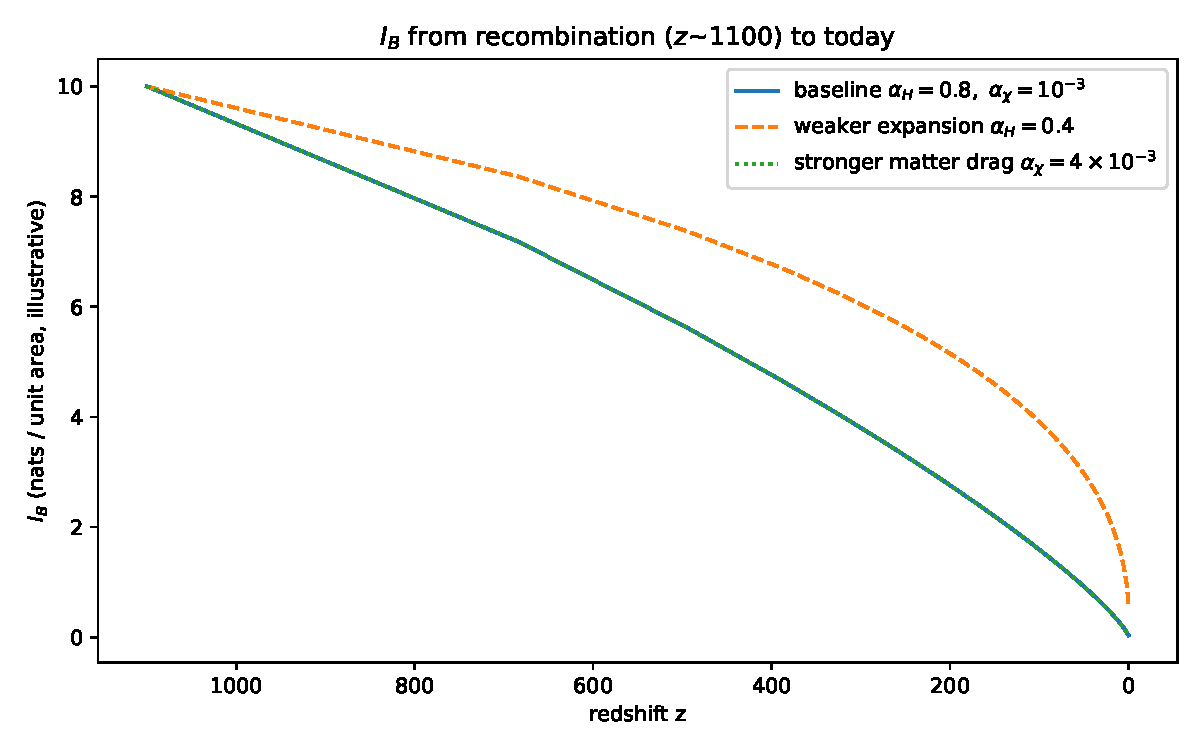
\includegraphics[width=0.78\textwidth]{ibudget_example_curves.pdf}
  \caption{Illustrative $I_B$ evolution from recombination to today for several coefficient choices. The redshift axis is inverted (left $\to$ early times).}
  \label{fig:ibudget}
\end{figure}
For standard $\Lambda$CDM cosmology, the $I_B$ evolution curve can be cross–referenced with known high–energy epochs to give approximate thresholds for phase transitions:

\begin{itemize}
  \item \textbf{Electroweak epoch} ($T\simeq 100\ \mathrm{GeV}$, $z\simeq 4\times 10^{15}$): $I_B \approx I_{B,\mathrm{EW}}$ where the budget first exceeds the index cost of electroweak–scale condensates.
  \item \textbf{QCD confinement} ($T\simeq 200\ \mathrm{MeV}$, $z\simeq 10^{12}$): $I_B \approx I_{B,\mathrm{QCD}}$ where color–charged condensates become kinematically accessible.
\end{itemize}

Here $I_{B,\mathrm{EW}}$ and $I_{B,\mathrm{QCD}}$ are computed by inserting the corresponding particle–structure index costs $\sum_a\ln(2j_a+1)$ into the budget–gating condition $\rho_I\le I_B(t)$. This provides a direct link between the abstract index budget and standard thermal–history milestones.

\subsection{Instability Timescale Bands}
From the linear analysis,
\[
  \tau_{\rm inst}\ \approx\ \frac{\chi}{D_I\,k_\ast^2}\ \sim\ \frac{\sigma}{D_I},
  \qquad
  k_\ast^2 \sim \chi^{-1}/\sigma,
\]
so the over-budget relaxation is governed by the ratio of the interfacial stiffness $\sigma$ to the mobility $D_I$ (both set by local rewrite physics). Figure~\ref{fig:tauinst} displays $\tau_{\rm inst}$ versus $D_I$ for representative $\sigma\in\{10^{-4},10^{-3},10^{-2}\}$ in arbitrary units. Once $\sigma$ and $D_I$ are tied to the singular spectrum of the one-cell transfer map, these curves translate into absolute times.

\begin{figure}[h]
  \centering
  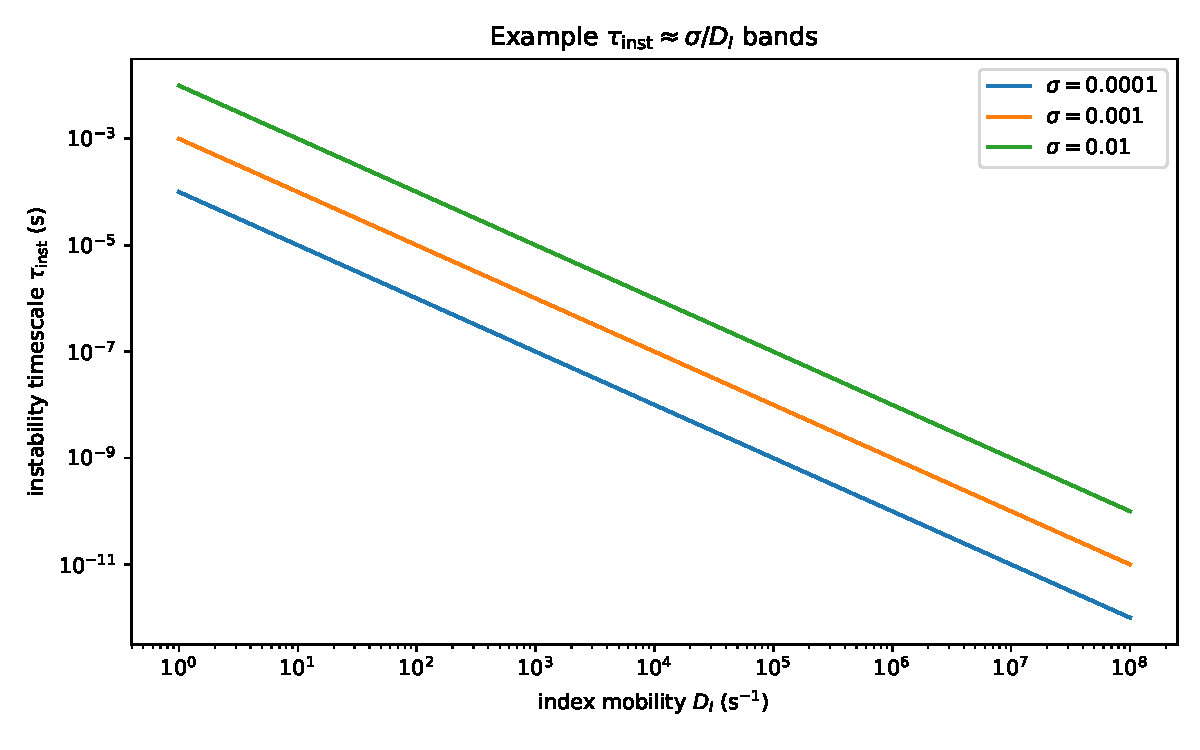
\includegraphics[width=0.72\textwidth]{inst_timescale_sweep.pdf}
  \caption{Example $\tau_{\rm inst}\approx \sigma/D_I$ bands for a sweep of mobilities $D_I$.}
  \label{fig:tauinst}
\end{figure}

\begin{figure}[h]
  \centering
  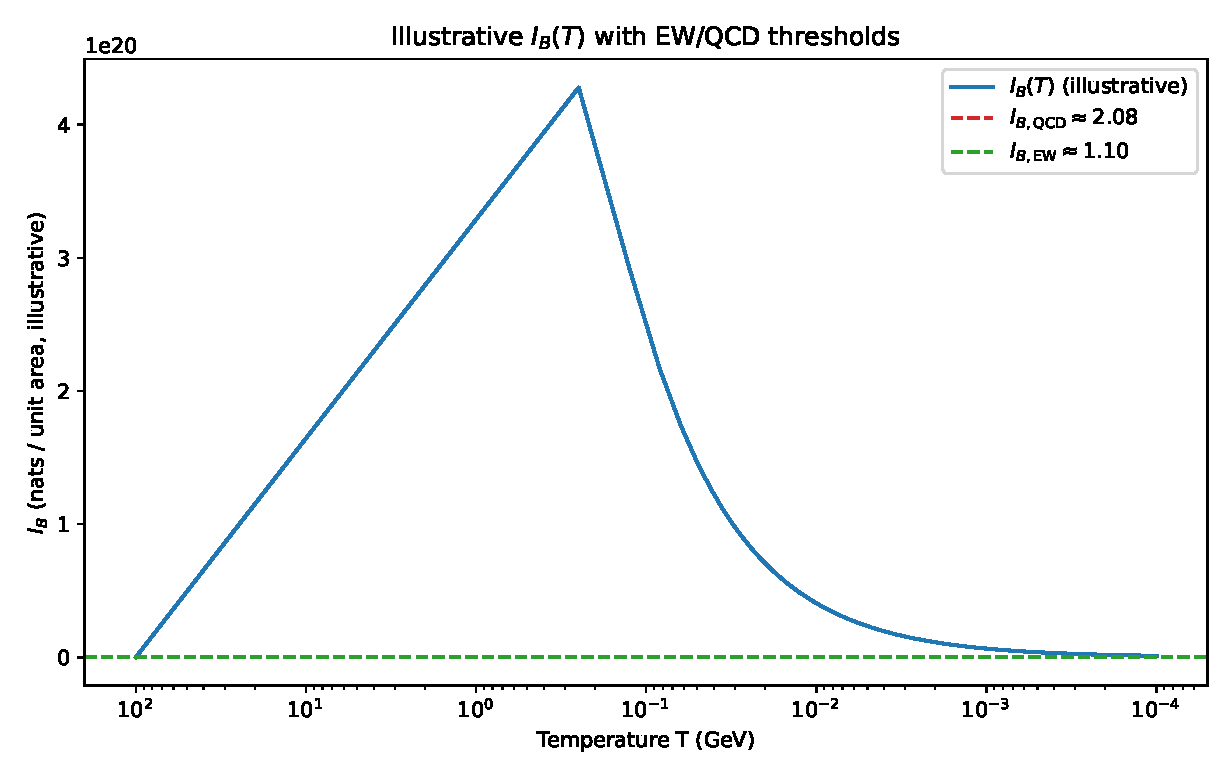
\includegraphics[width=0.78\textwidth]{ibudget_vs_temperature.pdf}
  \caption{Illustrative budget $I_B(T)$ from $T=100~\mathrm{GeV}$ to $100~\mathrm{keV}$ (log $T$ axis, inverted).
    Dashed lines mark the electroweak and QCD index thresholds,
    $I_{B,\mathrm{EW}}\approx 1.10$ and $I_{B,\mathrm{QCD}}\approx 2.08$.
    With the demo coefficients, $I_B(T)$ remains above both thresholds over this range;
    calibrating $(\alpha_H,\alpha_s,\alpha_\chi)$ to the one–cell transfer map moves the
  curve so that crossings occur at the desired epoch temperatures.}
  \label{fig:ibudget_vs_T}
\end{figure}

\subsection{Reproducibility}
The JSON file \texttt{ibudget_example_data.json} accompanying this appendix records the parameters, grids, and computed curves. The figures were generated by the script used to produce this appendix’s outputs.

\section*{References}
\begin{thebibliography}{99}
  \bibitem{bridge-monotonicity} M. Sandoz, ``Bridge-Monotonicity in Spin Networks,'' (2025), preprint.
  \bibitem{entropy-rewrites} M. Sandoz, ``Entropy Monotonicity via Local Graph Rewrites,'' (2025), preprint.
  \bibitem{operator-theory} M. Sandoz et al., ``Operator-Algebraic Perspective on Entropy Flow,'' (2025), preprint.
\end{thebibliography}

\end{document}
